The Standard Model of particle physics is one of the most precisely tested
theories. It is a relatistivic quantum field theory using the Lagrange
formalism.

It provides a unified description of three of the four forces of nature: the
electromagnetic interaction, the weak interaction, and the strong
interaction. Gravitation not included.

Natural units $\hbar = c = 1$. Can be recovered by dimensional
analysis. Heaviside--Lorentz units?

Einstein summation convention: Sum over repeated indices.

Space-time indices are given as greek letters. All other indices are latin.

The sign convention of the metric is $(+, -, -, -)$ (conventional in PP).

Cross-sections in barn $\SI{1}{\barn} = 10^{-28}\,\si{\metre\squared}$


The following summary of the theoretical foundation is based on
Refs.~\cite{Halzen:1984mc,Thomson:2013zua}.


\section{Particles and Interactions in the Standard Model}

The Standard Model, shown in~\Cref{fig:sm_particles}, consists of 12 elementary
spin-$\frac{1}{2}$ particles referred to as \emph{fermions} and their
anti-particles, and five types of particles with integer spin referred to as
\emph{bosons}. With the discovery of the Higgs boson in
2012~\cite{HIGG-2012-27,CMS-HIG-12-028}, experimental evidence for the existence
of all fermions and bosons predicted by the Standard Model is established.

\begin{figure}[htbp]
  \centering

  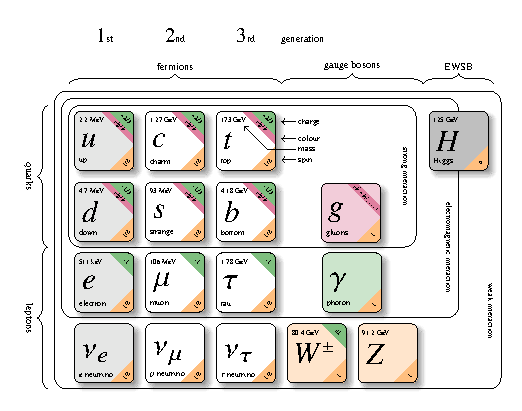
\includegraphics[width=\textwidth]{theory/sm}

  \caption{Particles of the SM. The diagram is adapted from Ref.~\cite{sm_tikz}
    with updated particle properties from Ref.~X. Antiparticles are not shown
    explicitly have additive quantum numbers of opposite sign but otherwise the
    same properties of the respective particle.}
  \label{fig:sm_particles}
\end{figure}


The elementary particles of the SM can be divided into three categories:
\begin{description}

\item[Fermions] predicted by the SM have spin-$\frac{1}{2}$. Consequently, they
  are massive\footnote{Neutrinos are considered as massless in the SM, however,
    the observation of neutrino
    oscillations~\cite{Super-Kamiokande:1998kpq,SNO:2002tuh} is experimental
    evidence for neutrinos having small but non-zero mass.} and adhere to the
  Pauli exclusion principle and are therefore considered to be \emph{matter}
  particles. For every fermions, a corresponding anti-particle exists that has
  the same properties but with opposite additive quantum numbers. The fermions
  of the SM are divided into \emph{quarks} that take part in the strong
  interaction and \emph{leptons} that do not. They are further divided into
  up-type quarks ($u$, $c$, $t$), down-type quarks ($d$, $s$, $b$), charged
  leptons ($e$, $\mu$, $\tau$), and neutrinos ($\nu_e$, $\nu_\mu$,
  $\nu_\tau$). The fermions of the SM come in three generations, the main
  difference between them being the mass of the fermions. All ordinary (stable)
  matter consists of fermions of the first generation: up-quarks, down-quarks,
  and electrons.

  The fermions carry charge-like quantum numbers that dictate the fundamental
  interactions they take part in. Quarks carry \emph{colour charge} which comes
  in three discrete values of either \emph{red}, \emph{green}, or \emph{blue},
  and the corresponding anti-colours for anti-quarks. Particles carrying colour
  charge take part in the strong interaction. Quarks and (electrically) charged
  leptons carry \emph{electric charge} and are therefore subject of the
  electromagnetic interaction. Fermions (anti-fermions) with left-handed
  (right-handed) chirality carry \emph{weak isospin} therefore taking part in
  charged-current weak interactions. All fermions carry \emph{weak hypercharge}
  and therefore take part in neutral current weak interactions.

\item[Gauge bosons] predicted by the SM are particles with spin-$1$ and are
  therefore also referred to as vector bosons. Gauge bosons are the quanta of
  fields arising in theories built on certain symmetry principles, referred to
  as gauge theories, which will discussed in
  \Cref{sec:theo_symmetries_interactions}. The gauge bosons mediate the three
  fundamental forces of nature through particle exchange.

  The (massless) gluons mediate the strong interaction through exchange of
  gluons between particles carrying colour charge. Gluons carry colour charge
  themselves and therefore couple to quarks or other gluons. The (massless)
  photon mediates the electromagnetic interaction between electrically charged
  particles. The gauge bosons of the weak interaction, the $W^\pm$ and $Z$
  bosons, take a special role in the SM since they are the only massive gauge
  bosons. The $W$ bosons are electrically charged and mediate the charged
  current weak interaction between particles carrying weak isospin. The
  uncharged $Z$ boson mediates the neutral-current weak interaction between
  particles carrying weak hypercharge.

\item[The Higgs boson] is the only scalar (spin-$0$) particle in the SM. The
  Higgs boson is a by-product of the Brout--Englert--Higgs (BEH)
  mechanism~\cite{Englert:1964et,Higgs:1964pj} that is used to include massive
  gauge bosons, the $W^\pm$ and $Z$ bosons, in the SM without violating the
  underlying principles of the gauge theory. This will be elaborated in
  \Cref{seq:theory_ewk}.

\end{description}


\section{Symmetries and Interactions}
\label{sec:theo_symmetries_interactions}

% \subsection{The Langrange Formalism}

The SM is a relativistic quantum field theory and thus described by space-time
dependent fields $\phi_i(\myvec{x})$. The dynamics of fields are given by the
\emph{Lagrangian density}, $\lagrange$, which is a function of the fields
$\phi_i$ and their space-time derivatives
$\partial_\mu \phi_i = \partial \phi_i / \partial x^\mu$ ($\mu = 0, 1, 2,
3$). The time-evolution of the fields follows from the principle of least
action, i.e.\ by minimising the action
$S = \int \mathrm{d}^4x \, \lagrange(\phi_i, \partial_\mu \phi_i)$, which yields
the the Euler--Lagrange equations
\begin{align*}
  \partial_{\mu} \left( \frac{\partial \lagrange}{\partial (\partial_{\mu} \phi_i)} \right) - \frac{\partial \lagrange}{\partial \phi_i} = 0
\end{align*} that provide the equations of motion for the fields. The Lagrangian density is
hereafter referred to as \emph{the Lagrangian}.

% \subsection{Local Gauge Invariance}

A continuous transformation of the fields that leaves the Lagrangian unchanged
is referred to as a \emph{gauge transformation}. The fields resulting from this
transformation follow the same equations of motion and thus describe the same
physical system. This invariance is referred to as \emph{gauge invariance} or
\emph{gauge symmetry}.
% An external observer cannot distinguish between fields related by gauge
% transformations and therefore the symmetry is considered an \emph{internal
% symmetry} of the theory.
The symmetry groups relevant for the description of the SM are the unitary group
of dimension one, $U(1)$, and the special unitary groups of dimension two and
three, $SU(2)$ and $SU(3)$, respectively. Any element of a unitary or special
unitary group can be written as
\begin{align*}
  \hat{U} = \exp\big[ i \theta_a G^a \big] \,\text{,}
\end{align*}
where $\theta_a$ are real parameters, $G^a$ are the generators of the group, and
summation over repeated indices is implied. A Lagrangian that is invariant to a
transformation $\hat{U}$ of the fields with parameters $\theta_a$ is said to
possess \emph{global} gauge invariance. The more restrictive case where the
Lagrangian is invariant with respect to transformations of the fields with
space-time dependent parameters $\theta_a(\myvec{x})$ is referred to as
\emph{local} gauge invariance.

This is illustrated in the case of the Lagrangian of the Dirac field of mass $m$
given by
\begin{align}
  \lagrange_{\text{Dirac}} = \bar{\psi} (i \gamma^\mu  \partial_\mu - m) \psi \,\text{,}
  \label{eq:dirac_lagrangian}
\end{align}
where $\psi$ ($\bar{\psi} = \psi^\dagger \gamma^0$) are (adjoint) Dirac spinors,
and $\gamma^\mu$ are the four Dirac matrices. \Cref{eq:dirac_lagrangian}
possesses global gauge invariance with respect to transformations from the
$U(1)$ group given by $\psi \to \psi^\prime = \exp[ i q \theta ] \psi$, where
$q$ is a coupling constant. However, when performing a local transformation by
letting the parameter be a function of space-time, i.e.\
$\theta \to \theta(\myvec{x})$, the invariance of the Lagrangian is spoiled due
to the derivative acting on the space-time dependent phase factor. One might
impose $U(1)$ local gauge invariance of the Lagrangian by adding terms to
\Cref{eq:dirac_lagrangian} that cancel the additional
contributions. Conventionally, this is done by substituting the derivative
$\partial_\mu$ by a gauge covariant derivative $D_\mu$ that transforms as
$D_\mu\psi \to \exp[ i q \theta(\myvec{x}) ] D_\mu\psi$ thus recovering local
gauge invariance. The definition of $D_\mu$ with these properties requires the
introduction of a new massless vector field, referred to as a \emph{gauge
  field}, with appropriate transformation properties:
\begin{align}
  D_\mu = \partial_\mu + i q A_\mu \qquad \text{with} \qquad A_\mu \xrightarrow{U(1)} A_\mu^\prime = A_\mu - \partial_\mu \theta(\myvec{x}) \,\text{.}
  \label{eq:covariant_derivative_qed}
\end{align}
The additional term introduced by substituting $\partial_\mu \to D_\mu$ in
\Cref{eq:dirac_lagrangian} is interpreted as an interaction between the fermion
and the vector boson of the gauge field.

The principle of local gauge invariance can be used to obtain the Lagrangian of
quantum electrodynamics (QED) describing electromagnetic interactions. The
symmetry group of QED is $U(1)_{Q}$, the subscript $Q$ indicating that the
elements of this group act on fields with electric charge. Imposing local gauge
invariance by substituting \Cref{eq:covariant_derivative_qed} into the Dirac
Lagrangian yields the interaction term
\begin{align*}
  \lagrange_{\text{int}} = - q \bar{\psi} \gamma^\mu \psi A_\mu \,\text{.}
\end{align*}
In the case of QED, the field $A^\mu$ is identified as the four-potential of the
electromagnetic field, and the coupling constant $q$ as the charge of the
fermion. Therefore, $\lagrange_{\text{int}}$ describes the coupling between the
photon and a fermion with electric charge $q$. For a single fermion type, the
Lagrangian of QED is given by
\begin{align*}
  \lagrange_{\text{QED}} = \underbrace{\lagrange_{\text{Dirac}}}_{\text{Free fermion field}}
  \quad\underbrace{- q \bar{\psi} \gamma^\mu \psi A_\mu}_{\text{Fermion--photon interaction}}
  \quad\underbrace{- \frac{1}{4} F_{\mu\nu} F^{\mu\nu}}_{\text{Free photon field}} \,\text{,}
\end{align*}
which additionally includes the Lagrangian of the free photon field defined by
the electromagnetic tensor given by
$F_{\mu\nu} = \partial_\mu A_\nu - \partial_\nu A_\mu$. The additional term also
fulfils the local gauge invariance with respect to $U(1)_Q$.

The principle of local gauge invariance is at the heart of the SM where it is
used to great success in describing the three fundamental interactions. The
symmetry group of the SM is
\begin{align*}
  SU(3)_{\text{color}} \otimes SU(2)_{\text{L}} \otimes U(1)_Y \,\text{,}
\end{align*}
where $SU(3)_{\text{color}}$ is the symmetry of the strong interaction, and
$SU(2)_{\text{L}} \otimes U(1)_Y$ the symmetry of the unified description of the
electromagnetic and weak interaction. These will be introduced in
\Cref{sec:theory_qcd} and \Cref{seq:theory_ewk}, respectively.

% \todo[inline]{Maybe note that a mass term a la $\frac{1}{2} m^2 A_\mu A^\mu$
%   would violate local gauge invariance.}

% \todo[inline]{Concluding remarks???}


\subsection{Quantum Chromodynamics}%
\label{sec:theory_qcd}

Quantum chromodynamics (QCD) is the quantum field theory describing the
interactions of quarks and gluons. The fundamental charge of QCD is colour
charge which comes in three distinct colors referred to as red, green, and blue
(r, g, b). The quark fields are consequently written in terms of the three
component objects
\begin{align*}
  \psi =
  \begin{pmatrix}
    q_\text{r} \\
    q_\text{g} \\
    q_\text{b}
  \end{pmatrix}
  \qquad
  \text{and}
  \qquad
  \bar{\psi} =
  \begin{pmatrix}
    \bar{q}_\text{r} & \bar{q}_\text{g} & \bar{q}_\text{b}
  \end{pmatrix} \,\text{,}
\end{align*}
in which the $q_i$ ($\bar{q}_i$) represent (adjoint) Dirac spinors describing
the quark field with color $i$. The strong interaction does not distinguish
between quarks of different colour thus a $SU(3)_{\text{colour}}$ is assigned,
the subscript indicating that elements of the group act in colour-space. The
generators of $SU(3)_{\text{colour}}$ are taken to be
\begin{align*}
  T_a = \frac{1}{2} \lambda_a \qquad \text{for} \qquad a = 1, \dots, 8 \,\text{,}
\end{align*}
where $\lambda_a$ are the Gell-Mann matrices.\footnote{Latin indices are raised
  and lowered according to $T_a = \delta_{ab} T^b$ or $T^a = \delta^{ab} T_b$,
  where $\delta$ refers to the Kronecker delta and the Einstein summation
  convention is adopted.} The theory of QCD is referred to as a Yang--Mills
gauge theory~\cite{Yang:1954ek} since the elements of $SU(3)_{\text{colour}}$ do
not commute in general, i.e.\ the symmetry group is non-Abelian. The commutation
relation between the generators is given by $[T_a, T_b] = i f_{abc} T^c$,
defining the structure constants $f_{abc}$ of the group.

Following the principle of local gauge invariance regarding a local
$SU(3)_{\text{color}}$ transformation
\begin{align*}
  \psi \to \psi^\prime = \exp[ i g_{\text{s}} \theta_a(\myvec{x}) T^a] \psi
  &&\bar{\psi} \to \bar{\psi}^\prime = \bar{\psi} \exp[ - i g_{\text{s}} \theta_a(\myvec{x}) T^a]  \,\text{,}
\end{align*}
where $g_{\text{s}}$ is referred to as the strong coupling constant, yields the
covariant derivative and eight massless gauge fields $G_\mu^a$
\begin{align*}
  D_\mu = \partial_\mu + i g_{\text{s}} G_\mu^a T_a
  \qquad \text{with} \qquad
  G_\mu^k \xrightarrow{SU(3)_{\text{colour}}} {G_\mu^k}^\prime = G_\mu^k  - \partial_\mu \theta^k(\myvec{x}) - g_{\text{s}} {f_{ij}}^k \theta^i(\myvec{x}) G_\mu^j \,\text{.}
\end{align*}
The gauge invariant kinetic term for the gluon fields is given by
\begin{align*}
  \lagrange_{G} = - \frac{1}{4} G_{\mu\nu}^{a} G^{\mu\nu}_{a}
\end{align*}
with the gluon field strength tensor
\begin{align*}
  G_{\mu\nu}^i = \partial_\mu G_\nu^i - \partial_\nu G_\mu^i - g_{\text{s}} {f^{i}}_{jk} G_\mu^j G_\nu ^k \,\text{.}
\end{align*}
The Lagrangian of QCD for a single flavour of quark with mass $m$ is
consequently given by
\begin{align}
  \lagrange_{\text{QCD}} =
  \underbrace{\bar{\psi} (i \gamma^\mu \partial_\mu - m) \psi}_{\text{Free quark field}}
  \underbrace{- g_{\text{s}} (\bar{\psi} \gamma^\mu T_a \psi) G_\mu^a}_{\text{Quark--gluon interactions}}
  \underbrace{- \frac{1}{4} G_{\mu\nu}^a G^{\mu\nu}_a}_{\text{Kinetic term}} \,\text{.}
  \label{eq:qcd_lagrangian}
\end{align}
This Lagrangian describes the free quark field, the interactions of quarks with
the eight gluons, and the kinetic energy contained in the gluon fields (the
kinetic term). The non-Abelian nature of the $SU(3)_{\text{colour}}$ group,
meaning a set of indices exists such that $f_{abc} \neq 0$, gives rise to the
distinct structure of QCD through the kinetic terms of the gluon fields in the
Lagrangian. These terms include self-interactions between gluons which
correspond to, in the language of Feynman diagrams, to triple and quartic gluon
vertices. Gluons themselves are carriers of colour charge, particularly a
combination of colour and anti-colour, which ultimately lead to such
behaviour. This is unlike the photon of QED which does not carry any electrical
charge and therefore does not couple to itself.


Two features of the theory of QCD are highlighted in the following:
\begin{description}

\item[Colour confinement] Due to the dynamics of the gluon self-interactions,
  free quarks or gluons cannot be observed in nature. Separating the quarks of a
  quark--antiquark pair leads to the formation of \emph{flux tubes} in the gluon
  field strength that result in a linear increase in field energy with
  separation of the quarks. Eventually, the energy stored in the gluon field is
  sufficiently large to create a quark--antiquark pair from the
  vacuum. Ultimately, only quarks (or gluons) bound into colourless composite
  particles (colour singlett states) remain. The most prevalent bound states of
  quarks are (anti-)baryons consisting of three (anti-)quarks, and mesons
  consisting of a quark--antiquark pair. The $SU(3)_{\text{colour}}$ symmetry
  also allows for colour singlett states of multiple gluons referred to as
  \emph{glueballs}, or other combinations of quarks such as tetra-
  ($q_1 \bar{q}_2 q_3 \bar{q}_4$) or pentaquarks ($q_1 q_2 q_3 q_4 \bar{q}_5$).

\item[Running coupling \& asymptotic freedom] The strong coupling constant,
  often expressed as $\alphas = g_{\text{s}}^2 / (4 \pi)$ in analogy to the
  fine-structure constant of QED $\alpha = e^2 / (4 \pi)$, is not constant but
  varies as a function of the momentum transfer, $q^2$, of an interaction. A
  quark scattering process involving the exchange of a gluon is represented by
  an infinite number of Feynman diagrams with different virtual corrections
  (e.g.\ quark or gluon loops). A process referred to as \emph{renormalisation}
  absorbs these corrections into an effective coupling constant, the coupling
  consequently becoming a function of $Q^2$. This effect occurs in both QED and
  QCD, however, with distinct signatures. While the coupling $\alpha(Q^2)$ of
  QED increases with $Q^2$, $\alphas(Q^2)$ of QCD decreases with $Q^2$ due to
  the gluon self-interaction. The high-$Q^2$ behaviour of the QCD coupling is
  referred to as asymptotic freedom. In addition, at sufficiently large $Q^2$
  the coupling is small such that perturbative methods can be used to obtain
  predictions.

\end{description}


\subsection{Theory of the Electroweak Interaction}%
\label{seq:theory_ewk}

The principle of local gauge invariance was previously used to generate the
fundamental interactions of QED and QCD. The characteristics of the weak
interaction make this approach more difficult. In particular, the mediators of
the interaction appear to be massive~\cite{pdg2020}
\begin{align*}
  m_W = \SI{80.377 +- 0.012}{\GeV} && m_{Z} = \SI{91.1876 +- 0.0021}{\GeV} \,\text{,}
\end{align*}
symmetry with respect to parity (space-inversion) transformations is
violated~\cite{Wu:1957my}, and charged-current interactions couple fermions of
different flavour that differ by one unit in electric charge. As a consequence,
the construction of a gauge theory of the weak interaction that respects gauge
invariance and describes the masses of gauge bosons and fermions requires
additional mechanisms that were not needed for the description of QED and QCD.


\subsubsection{Electroweak Unification}

The theory of the electroweak interaction was developed by Glashow, Salam, and
Weinberg in the 1960s to unify the electromagnetic and weak interaction in a
single model~\cite{Glashow:1961tr,Salam:1964ry,Weinberg:1967tq}. The electroweak
theory is constructed as a non-Abelian gauge theory based on a symmetry group
referred to as $SU(2)_{\text{L}} \otimes U(1)_{Y}$, the meaning of the indices
being illustrated in the following.

First, a new quantum number referred to as \emph{weak isospin}, $I$, with its
component along the 3-axis, $I_3$, is introduced. Based on the experimental
observation that the charged-current weak interaction only couples to particles
(antiparticles) with left-handed (right-handed) chirality, an appropriate
grouping of the SM fermions is chosen. In particular, left-handed fermions are
grouped into weak isospin doublets according to
\begin{align*}
  \begin{pmatrix}
    \nu_{e} \\
    e^{-}
  \end{pmatrix}_{\text{L}},
  \begin{pmatrix}
    \nu_{\mu} \\
    \mu^{-}
  \end{pmatrix}_{\text{L}},
  \begin{pmatrix}
    \nu_{\tau} \\
    \tau^{-}
  \end{pmatrix}_{\text{L}}
  \qquad
  \begin{pmatrix}
    u \\
    d^\prime
  \end{pmatrix}_{\text{L}},
  \begin{pmatrix}
    c \\
    s^\prime
  \end{pmatrix}_{\text{L}},
  \begin{pmatrix}
    t \\
    b^\prime
  \end{pmatrix}_{\text{L}}
  \qquad
  \text{with}
  \qquad
  I = \frac{1}{2}, I_3 = \pm \frac{1}{2} \,\text{,}
\end{align*}
the upper components corresponding to $I_3 = +\frac{1}{2}$, and nine singlet
states for right-handed fermions
\begin{align*}
  e^{-}_{\text{R}}, \mu^{-}_{\text{R}}, \tau^{-}_{\text{R}},
  u_{\text{R}}, d^\prime_{\text{R}}, c_{\text{R}}, s^\prime_{\text{R}}, t_{\text{R}}, b^\prime_{\text{R}}
  \qquad
  \text{with}
  \qquad
  I = 0, I_3 = 0 \,\text{,}
\end{align*}
where the indices L and R correspond to the separation of the fermion fields
into their left- and right-handed chiral components. The quark eigenstates of
the weak interaction are indicated by $d^\prime, s^\prime, b^\prime$ which are
related to the quark mass eigenstates via the Cabibbo--Kobayashi--Maskawa
matrix~\cite{Cabibbo:1963yz,Kobayashi:1973fv}. Right-handed neutrinos were
omitted since they are not part of the SM.\footnote{The determination of the
  nature of neutrinos is still an active area of physics research. In the SM,
  neutrinos are assumed to be massless which is in disagreement with the
  observation of neutrino oscillations. Under the assumption that neutrinos are
  Dirac particles, the non-vanishing mass would suggest that there is mixing
  between left- and right-handed chiral states of neutrinos. However, in the
  current theory right-handed neutrinos would be ``sterile'' meaning they would
  not interact via any of the interactions described by the SM. Alternative
  proposals are that neutrinos are not Dirac but Majorana
  particles~\cite{Majorana:1937vz}, which are particles that are identical to
  their antiparticles.} The subscript of the $SU(2)_{\text{L}}$ symmetry group
indicates that only the doublets of left-handed fermions mix under a
transformation from the group.\todo{If we are assuming massless quarks -> mass
  and weak eigenstates are the same.}

Second, a quantum number referred to as the \emph{weak hypercharge} defined
according to
\begin{align*}
  Y = 2 (Q - I_3) \,\text{,}
\end{align*}
where $Q$ refers to the electric charge, is introduced. Since the electric
charge differs between the upper and lower component of the $SU(2)_{\text{L}}$
doublets, a transformation of the group would violate the $U(1)_Q$ symmetry of
QED. This is remedied by replacing the $U(1)_Q$ with a $U(1)_Y$ symmetry with
$Y$ being defined such both components of the doublet have the same weak
hypercharge. The $U(1)_Q$ symmetry of QED will be recovered in a process called
electroweak symmetry breaking that will be introduced at a later point.


The principle of local gauge invariance with respect to the
$SU(2)_{\text{L}} \otimes U(1)_Y$ group is invoked to generate the interactions
of the electroweak theory. In the following, the weak isospin doublets are
denoted as $\chi_{\text{L}}$ and weak isospin singlets as $\psi_{\text{R}}$. The
gauge transformations with space-time dependent parameters $\alpha_a$
($a = 1, 2, 3$) and $\beta$ transform the fields as follows
\begin{align*}
  &\chi_{\text{L}} \to \chi_{\text{L}}^\prime = \exp\left[ i g \alpha_a(\myvec{x}) \frac{\sigma^a}{2} + i g^\prime \beta(\myvec{x}) \frac{Y}{2} \right] \chi_{\text{L}} \\
  &\psi_{\text{R}} \to \psi_{\text{R}}^\prime = \exp\left[ i g^\prime \beta(\myvec{x}) \frac{Y}{2} \right] \psi_{\text{R}} \,\text{,}
\end{align*}
where $g$ and $g^\prime$ are coupling constants, and $\sigma^a$ are the Pauli
matrices. The gauge covariant derivative is consequently given by
\begin{align*}
  D_\mu = \partial_\mu
  + i g W^a_\mu \frac{\sigma_a}{2}
  + i g^\prime B_\mu \frac{Y}{2} \,\text{,}
\end{align*}
where it is implied that the Pauli matrices only act on fields with left-handed
chirality. Furthermore, four gauge fields, $W_\mu^a$ for $a = 1, 2, 3$ and
$B_\mu$, are introduced which are associated to the $SU(2)_{\text{L}}$ and
$U(1)_Y$ symmetry, respectively. The gauge fields transform, in analogy to QED
and QCD, as follows
\begin{align*}
  W_\mu^k &\xrightarrow{SU(2)_{\text{L}} \otimes SU(1)_Y} {W_\mu^k}^\prime = W_\mu^k - \partial_\mu \alpha^{k}(\myvec{x}) - g {f_{ij}}^k \alpha^{i} W_\mu^j \\
  B_\mu   &\xrightarrow{SU(2)_{\text{L}} \otimes SU(1)_Y} {B_\mu}^\prime = B_\mu - \partial_\mu \beta(\myvec{x}) \,\text{,}
\end{align*}
where $f_{ijk}$ are the structure constants of the non-Abelian
$SU(2)_{\text{L}}$ group.

Substituting the gauge covariant derivative into the kinetic term of the Dirac
field yields the interaction Lagrangian of the electroweak interaction for left-
(L) and right-handed (R) chiral fields:
\begin{align}
  &\lagrange_{\text{int}}^{\text{L}} = i \bar{\chi}_{\text{L}} \gamma^\mu \left[i g W_\mu^a \frac{\sigma_a}{2} + i g^\prime B_\mu \frac{Y}{2} \right] \chi_{\text{L}} \label{eq:theory_electroweak_left} \\
  &\lagrange_{\text{int}}^{\text{R}} = i \bar{\psi}_{\text{R}} \gamma^\mu \left[i g^\prime B_\mu \frac{Y}{2} \right] \psi_{\text{R}} \,\text{.} \label{eq:theory_electroweak_right}
\end{align}
The four fields in the interaction Lagrangian are not the physical fields
observed in nature. The fields $W_\mu^1$ and $W_\mu^2$ are associated with
charged-current interactions noting that $\sigma_1$ and $\sigma_2$ are
anti-diagonal matrices. Similarly, $W_\mu^3$ is associated with a
neutral-current interaction coupling given $\sigma_3$ is a diagonal matrix.  The
physical fields of the charged-current interaction can be identified as
\begin{align*}
  W_\mu^\pm = \frac{1}{\sqrt{2}} (W_\mu^1 \mp i W_\mu^2)
\end{align*}
in analogy to the weak isospin ladder operators. Similarly, the physical fields
describing the neutral-current interactions via the exchange of $Z$ bosons and
photons can be expressed as a linear combination of the $W_\mu^3$ and $B_\mu$
gauge fields. Experimental results show that the $Z$ boson couples to both left-
and right-handed chiral states, although not equally, and therefore such a
mixing is required. The mixing can be described by a rotation of the fields by
the weak mixing angle $\theta_{\text{W}}$ according to
\begin{align*}
  \begin{pmatrix}
    A_\mu \\
    Z_\mu
  \end{pmatrix}
  =
  \begin{pmatrix}
    \cos\theta_{\text{W}} & \sin\theta_{\text{W}} \\
    -\sin\theta_{\text{W}} & \cos\theta_{\text{W}}
  \end{pmatrix}
  \begin{pmatrix}
    B_\mu \\
    W_\mu^3
  \end{pmatrix} \,\text{.}
\end{align*}
The weak mixing angle must be chosen such that
\Cref{eq:theory_electroweak_left,eq:theory_electroweak_right} reproduce the
coupling of QED, namely the photon must couple equally to left- and right-handed
particles with a coupling constant $e$. This yields the condition
\begin{align*}
  e = g \sin\theta_{\text{W}} = g^\prime \cos\theta_{\text{W}} \,\text{,}
\end{align*}\todo{Note ways to express sin / cos as a function of $g$ and $g^\prime$.}
connecting the QED coupling constant with the coupling constants $g$ and
$g^\prime$ of the electroweak unification. Conventionally, the couplings of the
electroweak unification are given in terms of $e$ and
$\sin^2\theta_{\text{W}} = \num{0.23124 +- 0.00004}$ at
$Q^2 = m_{Z}^2$~\cite{pdg2020}.

In analogy of QED and QCD, one adds the free field terms to the Lagrangian
\begin{align*}
  \lagrange_{W, Z, \gamma} =
  - \frac{1}{4} W_{\mu\nu}^a W^{\mu\nu}_a
  - \frac{1}{4} B_{\mu\nu} B^{\mu\nu}
\end{align*}
Since the $SU(2)_{\text{L}}$ group is non-Abelian, triple and quartic gauge
boson couplings are introduced into the theory.


\subsubsection{The Brout--Englert--Higgs Mechanism}

In the context of the electroweak theory, the non-zero masses of the gauge
bosons and the fermions have been ignored thus far. Explicitly adding a gauge
field mass term to the Lagrangian, which would take the form
\begin{align*}
  \lagrange_{\text{mass}}^{B} = -\frac{1}{2} m^2 B_\mu B^\mu
\end{align*}
for the $B_\mu$ gauge field (analogously for $W_\mu^a$), would violate
$SU(2)_{\text{L}} \otimes U(1)_Y$ symmetry due to the transformation properties
of the field. Similarly, fermion mass terms
\begin{align*}
  \lagrange_{\text{mass}}^{\text{fermion}} = - m \bar{\psi} \psi = - m [ \bar{\psi}_\text{R} \psi_\text{L} + \bar{\psi}_\text{L} \psi_\text{R} ]
\end{align*}
would lead to oscillations between left- ($\psi_{\text{L}}$) and right-handed
($\psi_{\text{R}}$) chiral states thus violating the $SU(2)_{\text{L}}$ symmetry
of the electroweak theory.

Concerning the masses of the gauge fields, a mechanism to dynamically generate
the required mass terms of the Lagrangian was introduced by Weinberg into the
electroweak theory~\cite{Weinberg:1967tq}. The mechanism traces back to Brout,
Englert, and Higgs~\cite{Englert:1964et,Higgs:1964pj} and is thus referred to as
the Brout--Englert--Higgs (BEH) mechanism.

The BEH mechanism introduces two complex scalar fields, one electrically charged
and one neutral field, arranged in a weak isospin doublet with $Y = 1$ according
to
\begin{align*}
  \phi =
  \begin{pmatrix}
    \phi^+ \\
    \phi^0
  \end{pmatrix}
  = \frac{1}{\sqrt{2}}
  \begin{pmatrix}
    \phi_1 + i \phi_2 \\
    \phi_3 + i \phi_4
  \end{pmatrix} \,\text{,}
\end{align*}
which can analogously be expressed as four real scalar fields $\phi_i$. The
Lagrangian of the complex scalar fields is given by the Klein--Gordon equation
\begin{align*}
  \lagrange = (\partial_\mu \phi)^\dagger (\partial^\mu \phi) - V(\phi)
\end{align*}
with the potential term of the fields denoted as $V(\phi)$. The aim of the BEH
mechanism is to embed the doublet of complex scalar fields in the electroweak
theory with a $SU(2)_{\text{L}}\otimes U(1)_Y$ symmetry. To fulfil the gauge
invariance of the electroweak theory, the potential can only depend on
$\phi^\dagger \phi$. One such choice is
\begin{align}
  V(\phi) = \mu^2 \phi^\dagger \phi + \lambda (\phi^\dagger \phi)^2
  \label{eq:higgs_potential}
\end{align}
with two parameters $\mu^2$ and $\lambda$.\footnote{On the grounds of
  renormalisability of the theory, the largest allowed power of
  $\phi^\dagger \phi$ in the potential term is two. TODO: Citation?} The
potential must be bound from below to have a well-defined state of minimum
potential energy (vacuum state) and therefore $\lambda$ must be positive. No
such restrictions exist for $\mu^2$, leaving two options. If $\mu^2 > 0$, the
vacuum state is $\phi = \myvec{0}$ and $\mu$ is related to the mass of the
scalar field. If $\mu^2 < 0$, the field configuration $\phi = \myvec{0}$ is at
an unstable point and the true vacuum is given by the condition
\begin{align*}
  \sum_{i = 1}^4 \phi_i^2 = -\frac{\mu^2}{\lambda} \eqqcolon v^2 \,\text{,}
\end{align*}
which represents a continuum of degenerate states at a radius of $v$ from the
origin in the space spanned by the four real scalar fields. The variable $v$ is
also referred to as the \emph{vacuum expectation value} (VEV). Hereafter, this
particular choice of potential is referred to as the Higgs potential. The choice
is further illustrated in \Cref{fig:mexican_hat} for a simplified model with
only a single complex scalar field.

\begin{figure}[htbp]
  \centering

  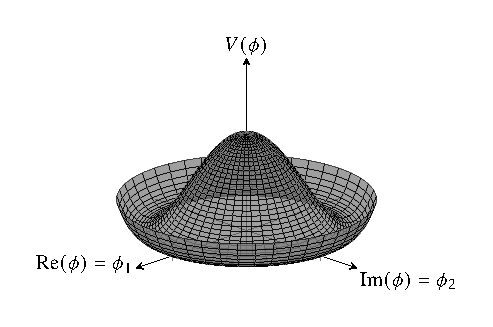
\includegraphics[width=0.55\textwidth]{theory/potential}

  \caption{The ``mexican-hat potential'' of a single complex scalar field as a
    lower dimensional example illustrating the choice of the Higgs potential in
    the SM. The degenerate vacuum states lie in a circle with radius $v$ given
    by the condition $\phi_1^2 + \phi_2^2 = v^2$. Adapted from
    Ref.~\cite{higgs_potential_tikz}.}%
  \label{fig:mexican_hat}
\end{figure}

The fields $\phi_i$ will assume a configuration that minimises the potential
energy, hence realising one of the infinite number of vacuum states. While the
full Lagrangian still possesses a $SU(2)_{\text{L}} \otimes U(1)_Y$ symmetry,
the spontaneous choice of a vacuum state with non-vanishing VEV appears to break
the symmetry, a process referred to as \emph{spontaneous symmetry
  breaking}. Perturbative methods have to be used to find solutions to the field
equations of motion, hence the fields have to be expressed as small
perturbations relative to a vacuum state. Let the vacuum state be
\begin{align*}
  \phi_{\text{v}} = \frac{1}{\sqrt{2}}
  \begin{pmatrix}
    0 \\
    v
  \end{pmatrix} \,\text{,}
\end{align*}
chosen such that only the neutral component is non-vanishing to ensure that the
$U(1)_Q$ symmetry of QED is recovered after spontaneous symmetry
breaking.\footnote{An infinitesimal $U(1)_Q$ transformation yields
  $(1 + i \epsilon Q) \phi_{\text{v}} = \phi_{\text{v}}$, thus leaving the
  vacuum state unchanged. This is not the case when replacing $Q$ with the
  generators of $SU(2)_{\text{L}}$ or $U(1)_Y$.} Four degrees of freedom for
perturbations relative to the chosen vaccum state exist. Three degrees of
freedom are chosen such that they leave $\phi^\dagger \phi$, and thus $V(\phi)$,
invariant. The remaining degree of freedom alters the value of
$\phi^\dagger \phi$ and therefore $V(\phi)$.\footnote{In the toy model depicted
  in \Cref{fig:mexican_hat}, the degrees of freedom correspond to perturbations
  of the vacuum state in angular and radial direction, respectively.} In the
Lagrangian describing the fields $\phi$, these perturbations appear as three
massless scalar fields and one massive scalar field. The quanta of the massless
fields are referred to as Nambu--Goldstone
bosons~\cite{Nambu:1960tm,Goldstone:1961eq}, however, a suitable gauge
transformation, referred to as the \emph{unitary gauge}, allows to remove the
massless scalar fields from the theory. In unitary gauge, the doublet of complex
scalar fields can be expressed as
\begin{align}
  \phi(\myvec{x}) = \frac{1}{\sqrt{2}}
  \begin{pmatrix}
    0 \\
    v + h(\myvec{x})
  \end{pmatrix}
  \label{eq:vacuum_state_perturb}
\end{align}
with $h(\myvec{x}) \in \mathbb{R}$.

Expressing the Higgs potential of \Cref{eq:higgs_potential} in terms of
perturbations of the vacuum state of \Cref{eq:vacuum_state_perturb} and dropping
terms not depending on $h(\myvec{x})$ yields
\begin{align*}
  V(h) =
  \lambda v^2 h(\myvec{x})^2
  + \lambda v h(\myvec{x})^3
  + \frac{\lambda}{4} h(\myvec{x})^4 \,\text{.}
\end{align*}
The first term of $V(h)$ represents the mass term of the scalar field $h$ with a
mass of $m_H = \sqrt{2\lambda} v$. The quantum of the scalar field is hereafter
referred to as the Higgs boson ($H$). The terms cubic and quadratic in the
scalar field represent self-interactions between Higgs bosons with constants
parameterising the coupling strengths defined according to
% \begin{align*}
%   g_{HHH} = \frac{3 m_{H}^2}{v} \qquad \text{and} \qquad g_{HHHH} = \frac{3 m_{H}^2}{v^2} \,\text{.}
% \end{align*}
\begin{align*}
  \lambda_{HHH} \coloneqq \lambda v = \frac{m_{H}^2}{2 v} \qquad \text{and} \qquad \lambda_{HHHH} \coloneqq \frac{\lambda}{4} = \frac{m_{H}^2}{8 v^2} \,\text{.}
\end{align*}
The Feynman vertices of Higgs boson self-interactions are depicted in
\Cref{fig:vertex_hhh,fig:vertex_hhhh}, respectively.

\begin{figure}[htbp]
  \centering

  \begin{subfigure}{0.33\textwidth}
    \centering
    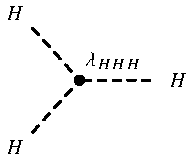
\includegraphics[scale=0.9]{feynman_graphs/higgs_hhh}
    \subcaption{}
    \label{fig:vertex_hhh}
  \end{subfigure}%
  \begin{subfigure}{0.33\textwidth}
    \centering
    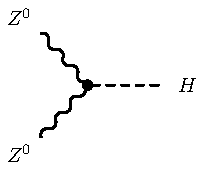
\includegraphics[scale=0.9]{feynman_graphs/higgs_hzz}
    \subcaption{}
  \end{subfigure}%
  \begin{subfigure}{0.33\textwidth}
    \centering
    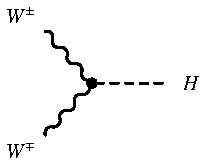
\includegraphics[scale=0.9]{feynman_graphs/higgs_hww}
    \subcaption{}
  \end{subfigure}

  \vspace{1em}

  \begin{subfigure}{0.33\textwidth}
    \centering
    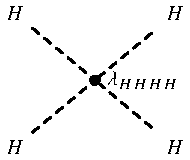
\includegraphics[scale=0.9]{feynman_graphs/higgs_hhhh}
    \subcaption{}
    \label{fig:vertex_hhhh}
  \end{subfigure}%
  \begin{subfigure}{0.33\textwidth}
    \centering
    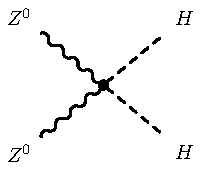
\includegraphics[scale=0.9]{feynman_graphs/higgs_hhzz}
    \subcaption{}
  \end{subfigure}%
  \begin{subfigure}{0.33\textwidth}
    \centering
    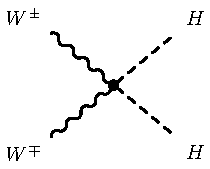
\includegraphics[scale=0.9]{feynman_graphs/higgs_hhww}
    \subcaption{}
  \end{subfigure}

  \caption{All vertices of Higgs bosons coupling to other bosons predicted by
    the SM.}%
  \label{fig:higgs_vertices}
\end{figure}

The terms of the Klein--Gordon equation involving the space-time derivatives
yield after substituting the $SU(2)_{\text{L}} \otimes U(1)_Y$ gauge covariant
derivative and inserting the physical fields describing the $W$ and $Z$ bosons:
\begin{align}
  (D_\mu \phi)^\dagger (D^\mu \phi) =
  \frac{1}{2} (\partial_\mu h) (\partial^\mu h)
  + \left[
  \frac{g^2 v^2}{4} W^{-}_\mu {W^{+}}^\mu
  +
  \frac{(g^2 + {g^\prime}^2) v^2}{8} Z_\mu Z^\mu
  \right] \left( 1 + \frac{1}{v} h \right)^2 \,\text{.}
  \label{eq:higgs_covariant_derivative}
\end{align}
The first term of \Cref{eq:higgs_covariant_derivative} yields the kinetic term
for the scalar field $h$. Moreover, the BEH mechanism dynamically generates mass
terms for the $W^\pm$ and $Z$ bosons while leaving the photon massless. Using
the four parameters of the electroweak theory (e.g.\ $g$, $g^\prime$, $m_{H}$,
$v$) the masses of the bosons can be obtained from the Lagrangian\footnote{TODO:
  Explain mysterious factor of two for the W mass term.}  such that
\begin{align*}
  &m_W = \frac{1}{2} g v  &&m_Z = \frac{1}{2} \sqrt{g^2 + {g^\prime}^2} \, v && m_A = 0 \,\text{.}
\end{align*}
Finally, \Cref{eq:higgs_covariant_derivative} describes interation vertices of
the form $WWH$, $ZZH$, $WWHH$, and $ZZHH$, which are depicted in
\Cref{fig:higgs_vertices}.


Prior to the discovery of the Higgs boson: Know $g$, $g^\prime$, and $v$ but not
$m_{H}$. After the Higgs boson was discovered, we now also know $m_H$ such that
the electroweak sector is fairly accurately specified.


\subsubsection{Fermion Masses}




\section{The Higgs Boson}


\clearpage

%%% Local Variables:
%%% mode: latex
%%% TeX-master: "../../phd_thesis"
%%% End:
